\documentclass{article}
\usepackage[margin=1in]{geometry}
\usepackage{graphics}
\usepackage{../common}
\usepackage{../pagesetup}
\usepackage{tikz}
\usetikzlibrary{bayesnet}


\begin{document}

\lecture{9}{October 2}{Sasha Rush}{Chris Hase, Denis Ellenrieder, Shuran Zheng, Rafi Small, Tim Menke}{Undirected Graphical Models}


\subsection{Left from last lecture: Conditional independence properties of DGMs}

When we have a directed graphical model (DGM), how can we ``read'' the graph and learn about the independence properties of the variables?
To begin we note that conditional independence follows if the marginal probability factors in the following way:
\begin{equation}
p(A,B|C) = p(A|C) \, p(B|C) \Rightarrow A \perp B | C
\end{equation}
Let \encircshaded{B} denote observing B, which informs our understanding on how $A$ and $C$ are conditional independent or not. Our cases are then:

\begin{align}
\encirc{A} \rightarrow \encirc{B} \rightarrow \encirc{C}, \; &A \perp C \; \crossmark \\
\encirc{A} \rightarrow \encircshaded{B} \rightarrow \encirc{C}, \; &A \perp C|B \; \checkmark \\
\encirc{A} \leftarrow \encirc{B} \rightarrow \encirc{C}, \; &A \perp C \; \crossmark \\
\encirc{A} \leftarrow \encircshaded{B} \rightarrow \encirc{C}, \; &A \perp C|B \; \checkmark \\
\encirc{A} \rightarrow \encirc{B} \leftarrow \encirc{C}, \; &A \perp C \; \checkmark \\
\encirc{A} \rightarrow \encircshaded{B} \leftarrow \encirc{C}, \; &A \perp C|B \; \crossmark \textrm{\ \ explaining away}
\end{align}
Information is being blocked in cases 2, 4, and 5 but flowing freely in all other cases.
It's useful to think about the concept of ``explaining away" to understand what is going on in the last case. '``Explaining away" is a common pattern of reasoning in which the confirmation of one cause of an observed or believed event reduces the need to invoke alternative causes.'\\(http://strategicreasoning.org/wp-content/uploads/2010/03/pami93.pdf)
\smallskip

How would a directed graphical model be interesting in practice?
One example is probabilistic programming: demonstrated in the IPython notebook ``DGM.ipynb".
The demonstration shows how we can convert programs from a directed to an undirected form. We can also specify priors on our features and visualize the flow of the model.
\smallskip

\emph{The purpose of creating a DGM is to specify the relationship between variables of interest, in order to to facilitate understanding of the independence properties.}

\subsection{Undirected Graphical Models (UGM)}

Differences of UGMs as opposed to DGMs:
\begin{enumerate}
	\item There are no arrows on lines
	\item No longer model \emph{local} probabilistic decisions (the term ``local" is important and defined later)
	\item UGMs are Markov random fields (similar to exponential families) or conditional random fields (similar to 		generalized linear models)
	\item Nice part: The rules are much simpler, especially for conditional independence
	\item Downside: The math is much more complicated
	\item Sasha's personal bias: UGMs are much more useful
\end{enumerate}


\subsubsection{Independence properties}

As stated above, we have conditional independence if the marginal probability factors in the following way:
\begin{equation}
p(A,B|C) = p(A|C) \, p(B|C) \Rightarrow A \perp B | C
\end{equation}

\begin{align}
\encirc{A} - \encirc{B} - \encirc{C}, \; &A \perp C \; \crossmark \\
\encirc{A} - \encircshaded{B} - \encirc{C}, \; &A \perp C|B \; \checkmark \\
\smallskip
\end{align}
We can say that we have ``conditional independence" between two nodes given some third node if all paths between the two nodes are blocked. For our simple example with three nodes, this is when the third node is in the evidence, that is, when the third node is ``seen''.
\smallskip

Here is an example of how independence works in the UGM.
\begin{center}
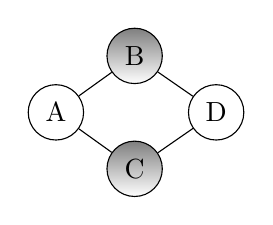
\begin{tikzpicture}

  \node (A) [latent] {A};
  \node (B) [shade, latent, above=of A, xshift=1cm, yshift=-1cm] {B};
  \node (C) [shade, latent, below=of A, xshift=1cm, yshift=1cm] {C};
  \node (D) [latent, right of=A, xshift=2cm] {D};

  \edge [-] {A} {B};
  \edge [-] {A} {C};
  \edge [-] {B} {D};
  \edge [-] {C} {D};

\end{tikzpicture}
\end{center}

\begin{align}
&A \perp D|S \; \text{if S blocks all the paths} \\
&\text{Here: } A \perp D|B,C \; \checkmark
\end{align}

\emph{Fundamental consequence:} Imagine we have a graph with a node $A$ and some complicated connection of nodes around $A$. 
We can make $A$ conditionally independent from all other nodes by conditioning on the ``Markov blanket" of $A$.
The Markov blanket is defined to be the \emph{neighbors of $A$}.
We will see later in this class that is is very nice if we can establish these independence properties.
We will be able to look at a point in a graphical model and, if we can condition on the Markov blanket of the node of interest, we can ignore the rest of the graph.
\smallskip

In the example below, conditioning on the Markov blanket of $A$ means conditioning on $B$, $C$, $E$, and $F$.

\begin{center}
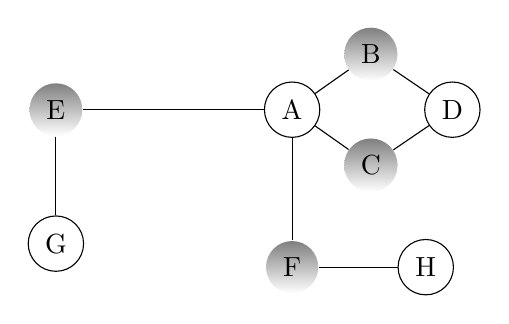
\begin{tikzpicture}

  \node (A) [latent] {A};
  \node (B) [shade,circle, above=of A, xshift=1cm, yshift=-1cm] {B};
  \node (C) [shade,circle, below=of A, xshift=1cm, yshift=1cm] {C};
  \node (D) [latent, right of=A, xshift=2cm] {D};
  \node (E) [shade,circle, left of=A, xshift=-2cm] {E};
  \node (F) [shade,circle, below of=A, yshift=-1cm] {F};
  \node (G) [latent, below=of E] {G};
  \node (H) [latent, right=of F] {H};

  \edge [-] {A} {B};
  \edge [-] {A} {C};
  \edge [-] {B} {D};
  \edge [-] {C} {D};
  \edge [-] {A} {E};
  \edge [-] {A} {F};
  \edge [-] {E} {G};
  \edge [-] {F} {H};

\end{tikzpicture}
\end{center}


\subsubsection{Converting directed to undirected graphs}

In order to convert directed to undirected graphs, we will use the (socially improperly termed) technique of \textit{moralization}, i.e. ``marry the parents".
\smallskip

\begin{center}
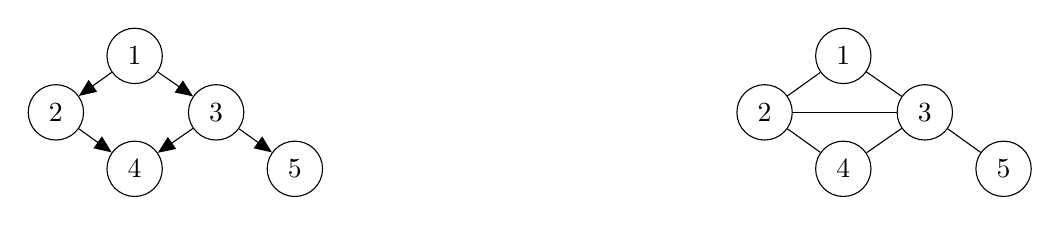
\begin{tikzpicture}

  \node (2) [latent] {2};
  \node (1) [latent, above=of 2, xshift=1cm, yshift=-1cm] {1};
  \node (4) [latent, below=of 2, xshift=1cm, yshift=1cm] {4};
  \node (3) [latent, right of=2, xshift=2cm] {3};
  \node (5) [latent, below=of 3, xshift=1cm, yshift=1cm] {5};

  \edge {1} {2};
  \edge {1} {3};
  \edge {2} {4};
  \edge {3} {4};
  \edge {3} {5};
  
  \node (2') [latent, xshift=9cm] {2};
  \node (1') [latent, above=of 2', xshift=1cm, yshift=-1cm] {1};
  \node (4') [latent, below=of 2', xshift=1cm, yshift=1cm] {4};
  \node (3') [latent, right of=2', xshift=2cm] {3};
  \node (5') [latent, below=of 3', xshift=1cm, yshift=1cm] {5};

  \edge [-] {1'} {2'};
  \edge [-] {1'} {3'};
  \edge [-] {2'} {4'};
  \edge [-] {3'} {4'};
  \edge [-] {3'} {5'};
  \edge [-] {2'} {3'};

\end{tikzpicture}
\end{center}

To carry out this process, we take all the directed edges and make them undirected. We then create additional edges by ``marrying'' the parents of a node. In this case we gain an extra edge between 2 and 3, which comes from marrying the parents of 4.
\smallskip
\\\\
Let's write Naive Bayes out in a directed graphical model:

\begin{center}
\begin{tikzpicture}
  %Define nodes
  \node[latent] (y) {$y$};
  \node[latent, below=of y, xshift=-1cm]  (x1) {$x_1$};
  \node[latent, below=of y, xshift=1cm]  (xv) {$x_V$};

  % Connect the nodes
  \edge {y} {x1};
  \edge {y} {xv};
  
  \path (x1) -- node[auto=false]{\ldots} (xv);
  
  %Define nodes
  \node[latent, xshift=10cm] (y') {$y$};
  \node[latent, below=of y', xshift=-1cm]  (x1') {$x_1$};
  \node[latent, below=of y', xshift=1cm]  (xv') {$x_V$};

  % Connect the nodes
  \edge [-] {y'} {x1'};
  \edge [-] {y'} {xv'};
  
  \path (x1') -- node[auto=false]{\ldots} (xv');

\end{tikzpicture}
\end{center}

For this case, the UGM and DGM are the same. However, if we condition the other way, i.e. the features $x_1, ..., x_D$ are on top of the DGM with directed arrows towards $y$ at the bottom, we would need to add connections in the UGM between all of the features. In the illustrated example, the joint probability having seen $y$ is
\begin{align}
\prod_d p(x_d) p(y|x_1,...,x_v).
\end{align}

\subsection{Corner cases}

Unfortunately, there are lots of corner cases in UGMs. DGMs and UGMs represent only a subset of all graphical models. There is some overlap between the UGM and DGM classes within the set of all independence structures. In the corner cases, we cannot convert between DGMs and UGMs and retain all of the independence information encoded within.

\begin{center}
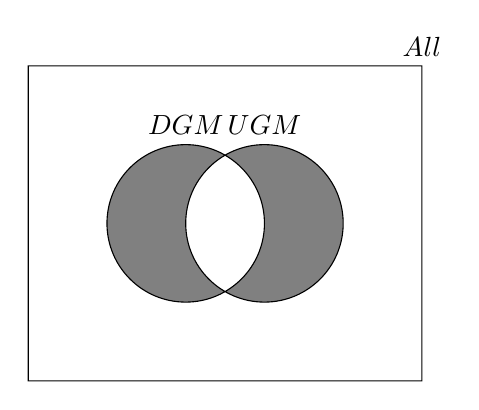
\begin{tikzpicture}[fill=gray]
% left hand
\scope
\clip (-2,-2) rectangle (2,2)
      (1,0) circle (1);
\fill (0,0) circle (1);
\endscope
% right hand
\scope
\clip (-2,-2) rectangle (2,2)
      (0,0) circle (1);
\fill (1,0) circle (1);
\endscope
% outline
\draw (0,0) circle (1) (0,1)  node [text=black,above] {$DGM$}
      (1,0) circle (1) (1,1)  node [text=black,above] {$UGM$}
      (-2,-2) rectangle (3,2) node [text=black,above] {$All$};
\end{tikzpicture}
\end{center}
\smallskip

We will now consider an example of a UGM and attempt to convert it to a DGM.
\begin{center}
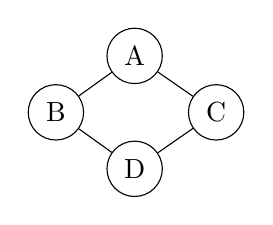
\begin{tikzpicture}

  \node (B) [latent] {B};
  \node (A) [latent, above=of B, xshift=1cm, yshift=-1cm] {A};
  \node (D) [latent, below=of B, xshift=1cm, yshift=1cm] {D};
  \node (C) [latent, right of=B, xshift=2cm] {C};

  \edge [-] {A} {B};
  \edge [-] {A} {C};
  \edge [-] {B} {D};
  \edge [-] {C} {D};

\end{tikzpicture}
\end{center}
Here we have
\begin{align}
A \perp D|B,C \; \checkmark\\
B \perp C|A,D \; \checkmark\\
\end{align}

One potential DGM we can create is
\begin{center}
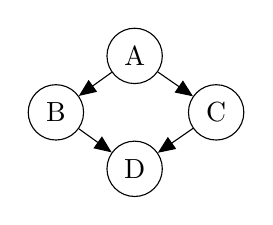
\begin{tikzpicture}

  \node (B) [latent] {B};
  \node (A) [latent, above=of B, xshift=1cm, yshift=-1cm] {A};
  \node (D) [latent, below=of B, xshift=1cm, yshift=1cm] {D};
  \node (C) [latent, right of=B, xshift=2cm] {C};

  \edge {A} {B};
  \edge {A} {C};
  \edge {B} {D};
  \edge {C} {D};

\end{tikzpicture}
\end{center}

In contrast to the UGM, the DGM has the following independence properties.
\begin{align}
&A \perp D|B,C \; \checkmark\\
&B \perp C|A,D \; \crossmark
\end{align}

Another DGM may be
\begin{center}
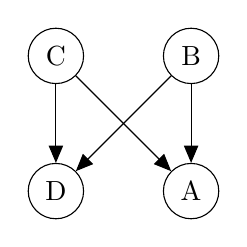
\begin{tikzpicture}

  \node (C) [latent] {C};
  \node (B) [latent, right=of C] {B};
  \node (D) [latent, below=of C] {D};
  \node (A) [latent, below=of B] {A};

  \edge {C} {D};
  \edge {C} {A};
  %\edge {C} {B};
  \edge {B} {D};
  \edge {B} {A};

\end{tikzpicture}
\end{center}
And now we see that
\begin{align}
&A \perp D|B,C \; \checkmark\\
&B \perp C|A,D \; \crossmark
\end{align}
So there is no directed graphical model structure that gives us same properties that the original UGM had.
\smallskip

How about another example of a DGM
\begin{center}
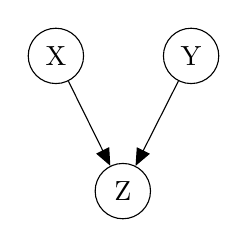
\begin{tikzpicture}

  \node (X) [latent] {X};
  \node (Y) [latent, right=of X] {Y};
  \node (Z) [latent, below=of X, xshift=0.85cm] {Z};

  \edge {X} {Z};
  \edge {Y} {Z};

\end{tikzpicture}
\end{center}
This graph has two properties:
\begin{align}
&(1) \; X \not\perp Y|Z \\
&(2) \; X \perp Y
\end{align}

\begin{center}
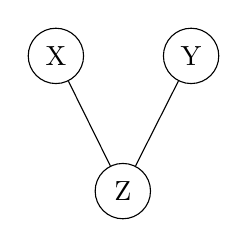
\begin{tikzpicture}

  \node (X) [latent] {X};
  \node (Y) [latent, right=of X] {Y};
  \node (Z) [latent, below=of X, xshift=0.85cm] {Z};

  \edge [-] {X} {Z};
  \edge [-] {Y} {Z};

\end{tikzpicture}
\end{center}
This graph has neither property 1 nor property 2.

\begin{center}
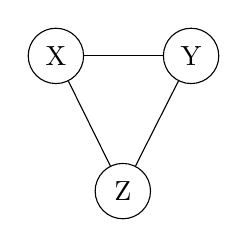
\begin{tikzpicture}

  \node (X) [latent] {X};
  \node (Y) [latent, right=of X] {Y};
  \node (Z) [latent, below=of X, xshift=0.85cm] {Z};

  \edge [-] {X} {Z};
  \edge [-] {Y} {Z};
  \edge [-] {X} {Y}

\end{tikzpicture}
\end{center}
Here we do have property 1 but not property 2.


\subsection{Parametrization of UGMs}

The following section is some of the harder material that we will cover. However, this is the last time we are introducing a new model. Thereafter, we will do inference on the models we have discussed.
\smallskip

\begin{center}
\begin{tikzpicture}

  \node (V) [latent] {A};
  \node (W) [latent, right=of X] {B};
  \node (X) [latent, below=of X, xshift=0.85cm] {C};
  \node (Y) [latent, right=of X, xshift=0.85cm] {D};
  \node (Z) [latent, below=of X, xshift=0.85cm] {E};

  \edge {V} {X};
  \edge {W} {X};
  \edge {X} {Y};
  \edge {X} {Z}
  
  \draw[red,thick,dashed] (0.9,-0.8) circle (1.5cm);
  \draw[blue,thick,dashed] (1,-2.5) circle (1.5cm);
  \node[draw] at (-1.5,0) {normal};
  \node[draw] at (-1.5,-3) {cat};

\end{tikzpicture}
\end{center}
Suppose that in this example the nodes within the red circle follow a local normal distribution, but that the nodes within the blue circle follow a local categorical distribution. The notation relating a node $X$ to its parents is $p(x|\text{pa}(x))$, where $\text{pa}(c)$ refers to the parents, and the conditional probability table is ``locally normalized", ``sums to one'', and is non-negative.
\smallskip

For UGMs we use ``global normalization". All is fine locally as long as the whole global probability sums up to make whole joint distribution normalized.
For this, we treat everything as an \emph{exponential family}.
\begin{align}
p(x_1, ..., x_d) = \text{multivariate exp. fam.} = \exp\left\{ \theta^T \phi(x_1, ..., x_D) - A(\theta) \right\}
\end{align}

Here, $\theta$ are the parameters and $\phi(x_1, ..., x_D)$ the sufficient statistics.
For every ``clique" in the graph, we associate a set of sufficient statistics. A ``clique" is defined as a set of nodes that are all connected to each other. Note: a set of one or two nodes forms a trivial clique.
\smallskip

In the discrete case:
\begin{align}
\phi(x_1, ..., x_D) = [ \phi_c(x_c) ...]^T
\end{align}
Each entry is an indicator of the value set for a clique. 

\begin{align}
\phi_c^v(x) = 
\begin{cases}
1 &\text{if clique } c \text{ has } x_c=v \\
0 &\text{otherwise}
\end{cases}
\end{align}

Suppose we have the following UGM in which each node can take on one of k possible discrete outcomes:
\begin{center}
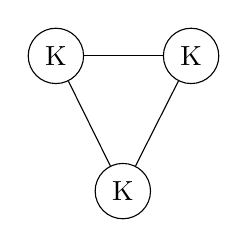
\begin{tikzpicture}

  \node (k1) [latent] {K};
  \node (k2) [latent, right=of k1] {K};
  \node (k3) [latent, below=of k1, xshift=0.85cm] {K};

  \edge [-] {k1} {k2};
  \edge [-] {k3} {k1};
  \edge [-] {k3} {k2};

\end{tikzpicture}
\end{center}
\smallskip

This means $ v \in K^3 $ in this example.
We also have a $\Theta$ associated with each of these values.
Since $\phi(x)$ is big (and awkward), we use the following notation:
\begin{align}
\theta^T \phi(x) = \sum_c \theta^T [0, ..., 0, \phi_c(x), 0, ...,]^T = \underbrace{\sum_c \theta_c(x_c)}_{\text{convenient notation}}
\end{align}

Now we write out the whole thing:
\begin{equation}
p(x_1, ..., x_D) = \exp \left\{ \underbrace{ \sum_c \theta_c (x_c) }_{\text{(neg) energy}} - A(\theta) \right\}
\end{equation}

Finally, we can compute the value $A(\theta)$:
\begin{align}
A(\theta) = \log \underbrace{\sum_{x'}}_\text{``everything"} \exp\{ \sum_c \theta_c (x'_c) \}
\end{align}
The sum over ``everything" is our nemesis because it is over something big. And in general, this is NP-Hard or even \#P-Hard. But in practice, the structure of the graph determines the difficulty. Examples of the ``everything'' include: all possible images, social network graphs... (How we can exchange the sums over $x'$ and $c$ depends on the structure of the graph.)

\subsection{Examples}

\subsubsection{Example 1: Naive Bayes model}

\begin{equation}
\encirc{A} - \encirc{B} - \encirc{C}, \; \text{all binary}
\end{equation}
We have two cliques: $\encirc{A}-\encirc{B}$ and $\encirc{B}-\encirc{C}$
\smallskip

Define features and parameters:
\begin{align}
\phi(x) =
	\begin{bmatrix}
		\mathbb{1}(A=0,B=0) \\
		\mathbb{1}(A=0,B=1) \\
		\mathbb{1}(A=1,B=0) \\
		\mathbb{1}(A=1,B=1) \\
		\mathbb{1}(B=0,C=0) \\
		\mathbb{1}(B=1,C=0) \\
		\mathbb{1}(B=0,C=1) \\
		\mathbb{1}(B=1,C=1)
	\end{bmatrix}, \;
\theta  =
	\begin{bmatrix}
	\theta_{AB}(0,0) \\
	\theta_{AB}(1,0) \\
	\theta_{AB}(0,1) \\
	\theta_{AB}(1,1) \\
	\theta_{BC}(0,0) \\
	\theta_{BC}(1,0) \\
	\theta_{BC}(0,1) \\
	\theta_{BC}(1,1)
	\end{bmatrix}
\end{align}

Then we have 
\begin{align}
p(A = a, B = b, C = c) = \exp\{\theta_{AB}(a,b) + \theta_{BC}(b,c) - A(\theta)\},
\end{align}
where $A(\theta) = \log\left(\sum_{a',b',c'} \exp\{\theta_{AB}(a',b') + \theta_{BC}(b',c')\}\right)$.

\subsubsection{Example 2: Hidden Markov model}
\begin{center}
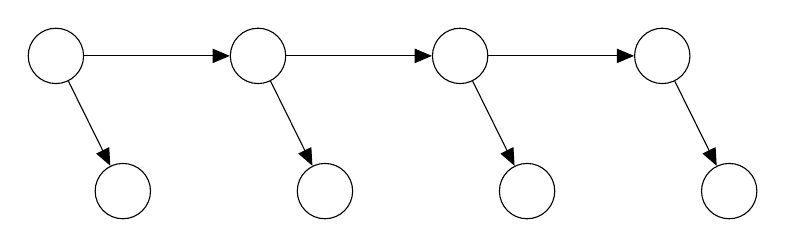
\begin{tikzpicture}

  \node (A) [latent] {};
  \node (B) [latent, right=of A, xshift=0.85cm] {};
  \node (C) [latent, right=of B, xshift=0.85cm] {};
  \node (D) [latent, right=of C, xshift=0.85cm] {};
  
  \node (A1) [latent, below=of A, xshift=0.85cm] {};
  \node (B1) [latent, below=of B, xshift=0.85cm] {};
  \node (C1) [latent, below=of C, xshift=0.85cm] {};
  \node (D1) [latent, below=of D, xshift=0.85cm] {};

  \edge {A} {B};
  \edge {B} {C};
  \edge {C} {D};

  \edge {A} {A1};
  \edge {B} {B1};
  \edge {C} {C1};
  \edge {D} {D1};

\end{tikzpicture}
\end{center}

\begin{center}
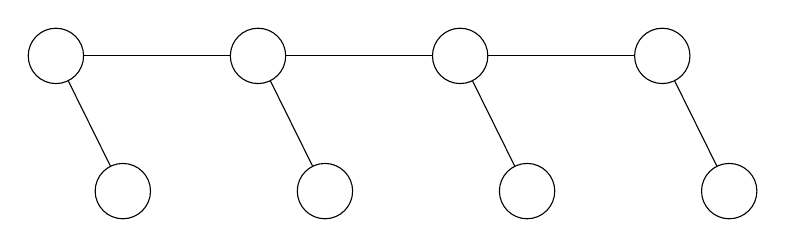
\begin{tikzpicture}

  \node (A) [latent] {};
  \node (B) [latent, right=of A, xshift=0.85cm] {};
  \node (C) [latent, right=of B, xshift=0.85cm] {};
  \node (D) [latent, right=of C, xshift=0.85cm] {};
  
  \node (A1) [latent, below=of A, xshift=0.85cm] {};
  \node (B1) [latent, below=of B, xshift=0.85cm] {};
  \node (C1) [latent, below=of C, xshift=0.85cm] {};
  \node (D1) [latent, below=of D, xshift=0.85cm] {};

  \edge [-] {A} {B};
  \edge [-] {B} {C};
  \edge [-] {C} {D};

  \edge [-] {A} {A1};
  \edge [-] {B} {B1};
  \edge [-] {C} {C1};
  \edge [-] {D} {D1};

\end{tikzpicture}
\end{center}
Any distribution obeying this structure has an exponential family parametrization.
We convert the local distribution
\begin{align}
p(y_1) \prod_i p(y_i | y_{i-1} ) p(x_i | y_i)
\end{align}
to the globally normalized distribution
\begin{align}
p(x,y) = \exp\{ \sum_i \left[\theta_{i,i-1}(y_i, y_{i-1}) +\theta_i(y_i, x_i)\right] - A(\theta) \}.
\end{align}


\subsubsection{Example 3: Ising model}

\begin{center}
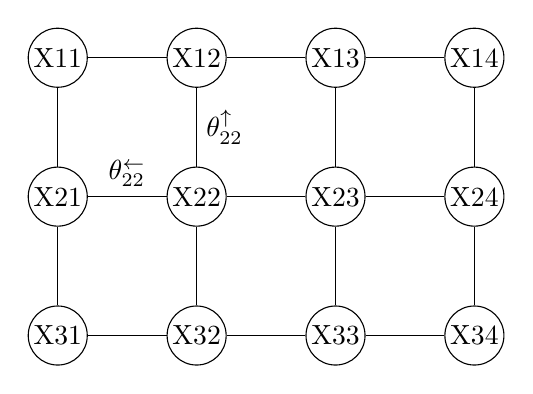
\begin{tikzpicture}

  \node (X11) [latent] {X11};
  \node (X12) [latent, right=of X11] {X12};
  \node (X13) [latent, right=of X12] {X13};
  \node (X14) [latent, right=of X13] {X14};
  \node (X21) [latent, below=of X11] {X21};
  \node (X22) [latent, right=of X21] {X22};
  \node (X23) [latent, right=of X22] {X23};
  \node (X24) [latent, right=of X23] {X24};
  \node (X31) [latent, below=of X21] {X31};
  \node (X32) [latent, right=of X31] {X32};
  \node (X33) [latent, right=of X32] {X33};
  \node (X34) [latent, right=of X33] {X34};

  \edge [-] {X11} {X12};
  \edge [-] {X12} {X13};
  \edge [-] {X13} {X14};
  \edge [-] {X11} {X21};
  \edge [-] {X12} {X22};
  \edge [-] {X13} {X23};
  \edge [-] {X14} {X24};
  \edge [-] {X21} {X22};
  \edge [-] {X22} {X23};
  \edge [-] {X23} {X24};
  \edge [-] {X21} {X31};
  \edge [-] {X22} {X32};
  \edge [-] {X23} {X33};
  \edge [-] {X24} {X34};
  \edge [-] {X31} {X32};
  \edge [-] {X32} {X33};
  \edge [-] {X33} {X34};
  
  \draw (X22) -- (X12) node [midway, right, sloped = false] (TextNode) {$\theta_{22}^{\uparrow}$};
  \draw (X22) -- (X21) node [midway, above, sloped] (TextNode) {$\theta_{22}^{\leftarrow}$};
  
\end{tikzpicture}
\end{center}
\smallskip
For this example, the shown grid could connect to other such grids. As an example, suppose we want to detect the foreground and background of an image. For this, we perform a binary classification of each pixel (0=pixel in background; 1=pixel in foreground). We want to obtain a probability that a pixel is in either class. The class should depend on the neighboring pixel so that there is consistency among neighboring pixels - it would be weird if every other pixel is in a different class.

This results in a binary model with neighbor scores. In order to force this to be a probability distribution, we treat the whole thing as an exponential family:
\begin{align}
p(x) = \exp\left\{ \sum_{ij} \left( \theta_{ij}^{\uparrow} (x_{ij}, x_{i-1,j} ) + \theta_{ij}^{\leftarrow} (x_{ij}, x_{i,j-1} ) + \theta_{ij}(x_{ij})\right) - A(\theta)\right\},
\end{align}
where $A(\theta) =  \log\left(\sum_{x'} \exp\sum_c \theta_c(x'_c)\right)$. Note that $A$ is again very hard to calculate. Also note that the ``missing'' $\theta_{22}^{\downarrow}$ and $\theta_{22}^{\rightarrow}$ in the diagram are given by other $\theta^{\uparrow}$ and $\theta^{\leftarrow}$ so that when we sum over all $i$ and $j$ we are not double counting any of the connections. 

\end{document}

